\documentclass[11 pt]{article}

\usepackage[utf8]{inputenc}
\usepackage[T1]{fontenc}
\usepackage[french]{babel}

\usepackage{amsmath}
\usepackage{empheq}
\usepackage{tikz}
\usepackage{tikz-qtree}
\usepackage{listings}
\usepackage{graphicx}
\usepackage{hyperref}

\usepackage[left=2cm,right=2cm,top=1.5cm,bottom=1.5cm]{geometry}

\title{Rapport de projet ISI-10:\\ AdaNet, Adaptive Neural Newtorks.}
\author{Serife Akkoyunlu, Luc Blassel, Romain Gautron}

\begin{document}
\maketitle
\section*{Introduction}
\paragraph{}Le but de ce projet est de reproduire les experiences et les methodes issues du papier suivant :\\
\href{https://arxiv.org/pdf/1607.01097.pdf}{C. Cortes, X. Gonzalvo, V. Kuznetsov, M. Mohri, S. Yang \emph{AdaNet: Adaptive Structural Learning of Artificial Neural Networks}}
En essayant de reproduire leur methode de construire des reseaux de neurones dont la structure est apprise et optimisee en meme temps que les poids, sur une tache de classification binaire issue du jeu de donnees d'images CIFAR-10.

\section{Comment marche AdaNet?}
\paragraph{}La structure du reseau est est generee. Le reseau entier qu'on appelera le reseau AdaNet, est augmente a chaque iteration par un sous reseau. Ce sous reseau est choisi en fonction de son effet sur une fonction objective pour pouvoir selectionner le meilleur sous reseau a rajouter au reseau Adanet a chaque etape. Pour bien comprendre le deroulement de ce processus on notera: $f_t$ le reseau AdaNet a l'etape $t$, $h_t$ et $h'_t$ les sous reseaux candidats (a l'etape $t$) avec pour chacun de ces sous reseaux $h_{t,k}$ la $k^{eme}$ couche du sous reseau et $h_{t,k,j}$ le $j_{eme}$ neurone de cette couche. $l$ est le nombre de couche maximale du sous reseau.
\paragraph{}L'algorithme se deroule alors selon ces etapes:
\begin{enumerate}
	\item \textbf{Initialisation du reseau: }On commence par generer les couches d'entree et de sortie.
	\item \textbf{Generation de sous-reseaux candidats: }On genere deux sous reseaux candidats\emph{(cf. Figure \ref{candidateModels})}:
	\begin{itemize}
		\item Un qui a une proofondeur identique au sous reseau genere precedement $\rightarrow k$
		\item Un qui augmente la profondeur de 1 par rapport au sous reseau precedent $\rightarrow k+1$
	\end{itemize}
	Ces deux sous reseaux obeissent aux memes regles de connectivite. C'est a dire que le premiere couche du reseau du sous reseau $h_t$  est reliee a la couche d'entree de $f_t$, la derniere couche $h_{t,l}$ du sous reseau est forcement connectee a la couche de sortie de $f_t$. Pour les couches intermediaires, chaque couche $h_{t,k}$ est forcement reliee a $h_{t,k-1}$ et peut etre reliee aux couches de niveau precedent dans tous les sous reseaux precedement generes, c'est a dire $h_{t\in[1,t-1],k-1}$.
	\emph{Lors de la premiere iteration il faut forcement choisir le sous reseau qui augmente la profondeur puisque $k=0$}
	\item \textbf{Choix du sous-reseau: }Parmi ces deux sous reseaux candidats $\mathbf{h}$ et $\mathbf{h'}$ on choisit celui qui, apres un entrainement, minimise le plus la fonction objective suivante:
	\begin{equation*}
		F_t(\mathbf{w,h})=\frac{1}{m}\sum^m_{i=1}\Phi(1-y_if_{t-1}(x_i)-y_i\mathbf{w\cdot h}(x_i)) + \mathcal{R}(\mathbf{w,h})
	\end{equation*}
	Avec $x_i$ les exemples d'entrainement, $y_i$ les reponses attendues, $m$ Le nombre d'exemples,$\mathbf{w}$ Les poids associes au sous reseau candidat $\mathbf{h}$ et $\Phi$ une fonction (soit la fonction exponentielle soit la fonction logistique). Le terme $\mathcal{R}(\mathbf{w,h})$ est un terme de regularisation qui est laisse a $0$ lors des experimentations.\\
	Si $F(\mathbf{w,h})>F(\mathbf{w,h'})$ alors le sous reseau candidat $\mathbf{h'}$ est choisi et $\mathbf{h}_t \leftarrow \mathbf{h'}$\\
	\item \textbf{Condition d'arret: }Une fois que le meilleur sous reseau est selectionne on regarde si celui ci a apporte une amelioration au reeseau AdaNet. Si la fonction objective de l'entrainement de $f_{t-1}$ \emph{(qui n'est pas le meme que celle utilisee pour le choix du meilleur sous reseau)} est meilleure avec le sous reseau alors que sans alors: $f_t \leftarrow f_{t-1}+\mathbf{w}^*\mathbf(h)_t$ sinon l'integration du sous reseau n'apporte rien de plus au reseau $f_{t-1}$ et celui est retourne, terminant alors l'execution de l'algorithme. Si cette condition d'arret n'est jamais verifiee, l'elrogithme s'arrete au bout de $T$ iteration et retourne le reseau $f_T$
\end{enumerate}
\paragraph{}On voit donc bien que la generation et l'ajustement des poids du reseau se fait iterativement a chaque etape.\\ \bigskip
\begin{figure}[h]
	\centering
	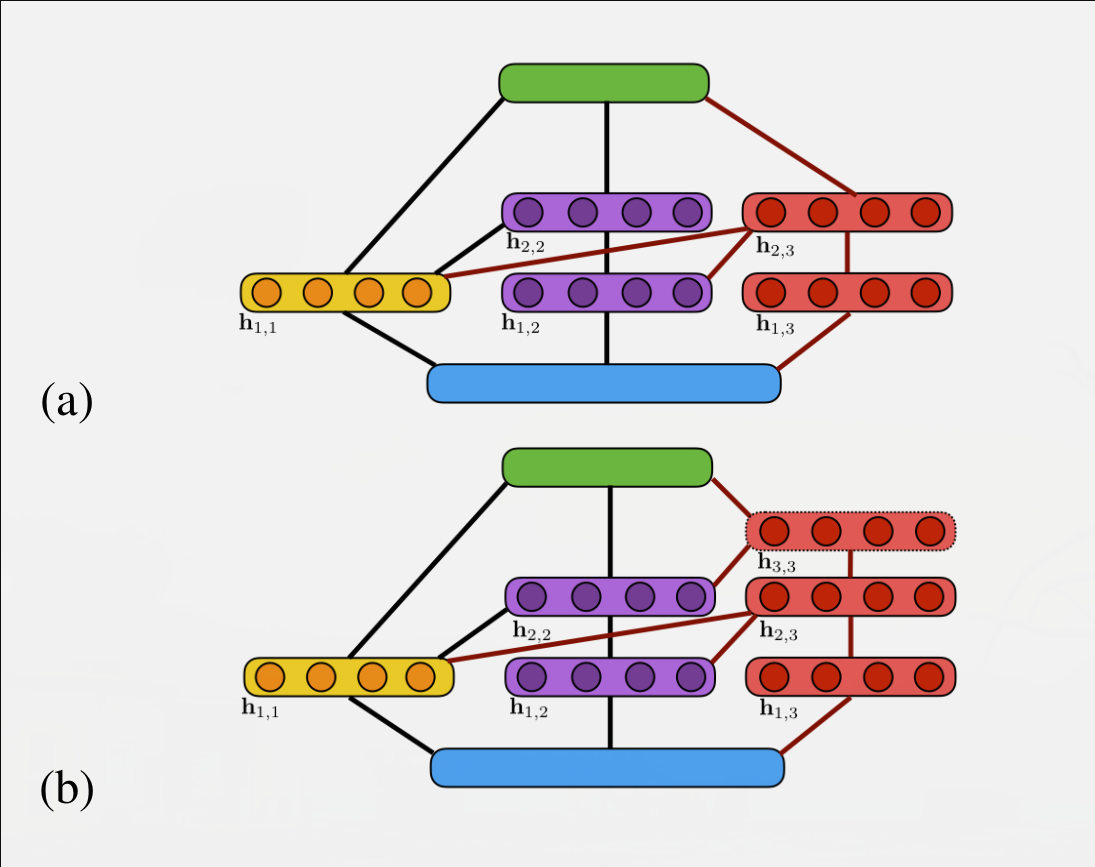
\includegraphics[width=0.5\textwidth]{schema.png}
	\caption{Les deux sous reseaux candidats generes a l'etape $3$ (en rouge), un de profondeur $k=2$ comme le sous reseau choicit a l'etape precedente (en bleu), et un de profondeur $k=3$ qui augmente la profondeur generale de $1$. Ce sont ces deux reseaux AdaNets potentiels qui vont etre evalues}
	\label{candidateModels}
\end{figure}



\section{Notre implementation}
\section{Resultats}
\section{Pistes futures}





\end{document}
